\section{Zmienne losowe o zadanym rozkładzie}
\subsection{Metoda transformacji}
\begin{frame}{Zmienne losowe o zadanym rozkładzie\linebreak Metoda transformacji}
	\begin{block}{Podstawowe generatory - o rozkładzie równomiernym (uniform deviate):}
		\[
			P\left\{x < X < x + dx\right\} = p(x)dx = \begin{cases}
				dx,\hspace{0.5cm} 0 < x < 1\\
				0,\hspace{0.65cm} $ gdzie indziej$
			\end{cases}
		\]
		\[
			\fbox{$p(x) = 1$}
		\]
	\end{block}
\end{frame}
%%%%%%%%%%%%%%%
\begin{frame}{Metoda transformacji}
	\begin{block}{Generatory zmiennej losowej $y(x)$ o \textit{zadanym rozkładzie}
	$p(y)$:}
	\[
		\lvert p(y)dy \rvert \hspace{0.1cm} = \hspace{0.1cm} \lvert p(x)dx \rvert \hspace{6.8cm}
	\]
	\[
		\phantom{x} \hspace{0.2cm} p(y) \hspace{0.1cm} = \hspace{0.1cm} p(x) \left| \frac{dx}{dy} \right| \Rightarrow p(y) = \frac{dx}{dy}, \hspace{0.1cm} x = F(y) = \int_{0}^{y} p(y)dy
	\]
	\[
		\fbox{$y(x) = F^{-1}(x)$} \text{ ,} \hspace{1cm} F(y) - \text{dystrybuanta rozkładu p(y)}
	\]
	\end{block}
	\vspace{1cm}
	
	\flushright \textit{Zadanie: } rozkład wykładniczy $p(y) = e^{-y}$
\end{frame}
%%%%%%%%%%%%%%
\begin{frame}{Zmienne o rozkładzie normalnym}
	\centering 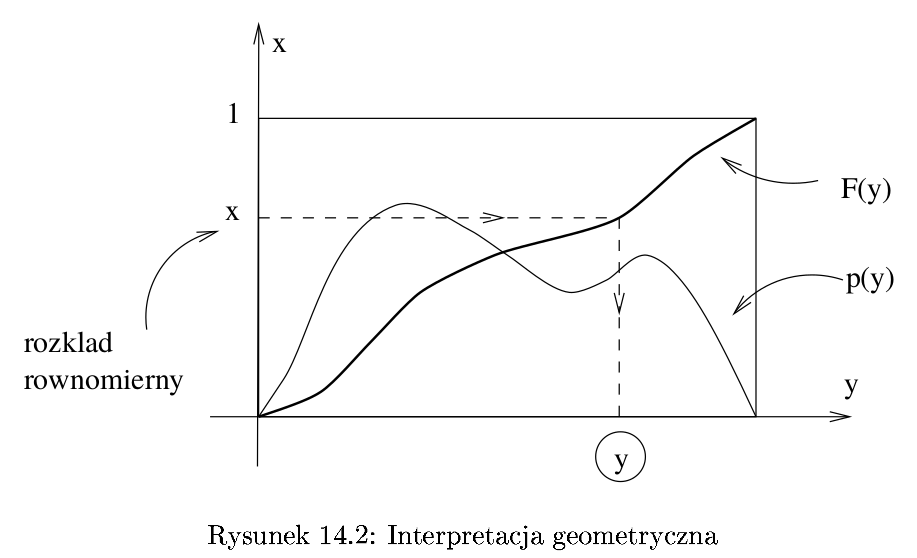
\includegraphics[width=1\linewidth]{img/14/14_6_1_img.png}
\end{frame}
%%%%%%%%%%%%%%
\subsection{Zmienne o rozkładzie normalnym}
\begin{frame}{Zmienne o rozkładzie normalnym}
	\begin{block}{Uogólnienie met. transformacji dla n-D}
		$x_{1},x_{2},\ldots,x_{n}$ - zmienne o łącznym rozkładzie $p(x_{1},x_{2},\ldots,x_{n})dx_{1} \ldots dx_{n}$\\
		\vspace{0.5cm}
		$y_{1},y_{2},\ldots,y_{n}$ - każda $y$ - funkcja wszystkich $x$, tyle samo $x$ i $y$
	\end{block}
\end{frame}

%%%%%%%%%%%%%%
\begin{frame}{Zmienne o rozkładzie normalnym}
	\begin{block}{łączny rozkład prawdopodobieństwa $y$:}
		\[
			p(y_{1},y_{2},\ldots,y_{n})dy_{1}dy_{2} \ldots dy_{n} =
		\]
		\[
			= p(x_{1},x_{2},\ldots,x_{n}) \underbrace{\left|\frac{\partial(x_{1},x_{2},\ldots,x_{n})}{\partial(y_{1},y_{2},\ldots,y_{n})}\right| dy_{1}dy_{2} \ldots dy_{n}}_{dx_{1}dx_{2} \ldots dx_{n}}
		\]
	\end{block}
\end{frame}
%%%%%%%%%%%%%%
\begin{frame}{Metoda Box-Muller (1958)}
	\begin{block}{Metoda Box-Muller (1958) generacji zmiennych losowych o rozkładzie normalnym}
		\[
			p(y)dy = \frac{1}{\sqrt{2\pi}}e^{-\frac{y^{2}}{2}}dy \quad, \qquad \text{r. } N(0,1)
		\]
		$x_{1}, x_{2}$ - zm. losowe niezależne, rozkł. równomierny na $(0, 1)$
	\end{block}

	\begin{block}{transformacja:}
		\[
			y_{1} = \sqrt{-2 \ln(x_{1})} \cos(2\pi x_{2})
		\]
		\[
			y_{2} = \sqrt{-2 \ln(x_{1})} \sin(2\pi x_{2})
		\]
	\end{block}
\end{frame}
%%%%%%%%%%%%%%
\begin{frame}{Metoda Box-Muller (1958)}
	\begin{block}{stąd:}
		\[
			x_{1} = \left[- \frac{1}{2} (y_{1}^{2} + y_{2}^{2})\right]
		\]
		\[
			x_{2} = \frac{1}{2\pi} \arctan\frac{y_{1}}{y_{2}}
		\]
	\end{block}
	
	\begin{block}{co daje:}
		\[
			\frac{\partial(x_{1}, x_{2})}{\partial(y_{1}, y_{2})} = \begin{vmatrix}
				\frac{\partial x_{1}}{\partial y_{1}} & \frac{\partial x_{1}}{\partial y_{2}} \\
				\frac{\partial x_{2}}{\partial y_{1}} & \frac{\partial x_{2}}{\partial y_{2}}
			\end{vmatrix} =
			- \left[\frac{1}{\sqrt{2\pi}} e^{-\frac{y_{1}^{2}}{2}}\right] \left[\frac{1}{\sqrt{2\pi}} e^{-\frac{y_{2}^{2}}{2}}\right]
		\]
		$\Rightarrow$ $y_{1} y_{2}$ - każda oddzielnie ma rozkład normalny (2 niezależne!)
	\end{block}
\end{frame}
%%%%%%%%%%%%%%
\begin{frame}{Uproszczenie obliczeń}
	\begin{block}{Zamiast:}
		$x_{1}, x_{2}$ - rozkład równomierny w jednostkowym kwadracie
	\end{block}

	\begin{block}{bierzemy:}
		$v_{1}, v_{2}$ - współrz. punktu w jednostkowym kole:\\
		$v_{1}^{2} + v_{2}^{2} < 1$,\\
		$R = v_{1}^{2} + v_{2}^{2}$ - ma rozkład równomierny - zamiast $x_{1}$\\
		$\angle(v_{1}, v_{2})$ - zamiast $x_{2}$
		\[
			\cos(2\pi x_{2}) = \frac{v_{1}}{\sqrt{R}}; \qquad \sin(2\pi x_{2}) = \frac{v_{2}}{\sqrt{R}}
		\]
		i tak unikamy stosowania funkcji trygonometrycznych
	\end{block}
\end{frame}
%%%%%%%%%%%%%%
\begin{frame}{Uproszczenie obliczeń}
	\begin{block}{}
		\[
			y_{1} = v_{1}\sqrt{\frac{-2 \ln(v_{1}^{2} + v_{2}^{2})}{v_{1}^{2} + v_{2}^{2}}},
		\]
		\[
			y_{2} = y_{1} \cdot \frac{v_{2}}{v_{1}}
		\]
		$y_{1}, y_{2}$ - niezależne, obie o $N(0,1)$
	\end{block}

	\vspace{0.5cm}
	\begin{flushright}
		\textit{Zadanie}
	\end{flushright}

	\vspace{-0.5cm}
	``Numerical Recipes'' rozkłady:
	\begin{itemize}
		\item gamma
		\item Poissona
		\item binominalny (``rejection method'' 7.3)
	\end{itemize}
\end{frame}